\documentclass[12pt, a4paper]{article}
\usepackage{float}
\usepackage[utf8]{inputenc}
\usepackage[T1]{fontenc}
\usepackage{newtxtext,newtxmath} % Times New Roman equivalent font in LaTeX
\usepackage[top=2cm, bottom=2.5cm, left=3cm, right=1.5cm]{geometry}
\usepackage{graphicx}
\usepackage{amsmath}
\usepackage{booktabs}
\usepackage{indentfirst}
\usepackage{caption}
\usepackage{hyperref}

% Page and document settings to match AITU template specifications
\setlength{\parindent}{1.25cm}
\renewcommand{\baselinestretch}{1.0}
\captionsetup[figure]{font=small,labelfont=bf,justification=centering,name={Fig.}}
\captionsetup[table]{font=small,labelfont=bf,position=top,justification=justified}

% Ensure section headers match standard formatting style
\usepackage{titlesec}
\titleformat{\section}{\normalfont\fontsize{12}{14}\bfseries}{\thesection}{1em}{}
\titleformat{\subsection}{\normalfont\fontsize{12}{14}\itshape}{\thesubsection}{1em}{}

\title{TASK-AWARE EVALUATION OF JPEG RECOMPRESSION AND RGB BIT-DEPTH REDUCTION FOR OBJECT DETECTION}

\author{
  \textbf{Amir Karataev} \\
  \small Master of Science, Graduate Student, School of Software Engineering \\
  \small amirkarataev1501@gmail.com, ORCID: 0009-0007-7074-6421 \\
  \small Astana IT University, Kazakhstan \\
  \textbf{Shynar Akhmetzhanova} \\
  \small Candidate of Technical Sciences, Assistant Professor, School of Software Engineering \\
  \small Sh.Akhmetzhanova@astanait.edu.kz, ORCID: 0000-0002-4131-8328 \\
  \small Astana IT University, Kazakhstan
}

\date{}

\begin{document}

\maketitle

\begin{abstract}
How does image storage affect object detection? Traditional image quality metrics typically focus on human vision. However, computer vision models see images very differently. To explore this difference, we ran tests on the COCO val2017 dataset using two different compression methods. On one hand, we applied JPEG recompression with different quality levels (94, 88, 75, 50, and 25). On the other hand, we uniformly reduced the bit depth of each RGB color channel, storing the output as 24-bit PNG files with a bit depth simulating a reduction from 8 bits to one bit per channel. We processed each resulting image using the standard YOLOv8n detector. Our analysis tracked memory footprint, traditional visual fidelity, and actual detection accuracy. 
The results show that JPEG recompression performs remarkably well in balancing the tradeoff between memory footprint and accuracy. Reducing the dataset size using quality level 88 reduced the total size by a factor of 2.02 (leaving only 384.22 MB of data), while causing a barely noticeable decrease in mAP50 by 0.77\% (from 0.5187 to 0.5147). In contrast, using PNG containers for quantized RGB data proved to be highly inefficient. Although 7-bit quantization preserved the baseline accuracy (mAP50 = 0.5189), the physical file size increased to 1912.67 MB. Reducing quantization significantly degraded the detector's performance. At 3 bits per channel, mAP50 dropped by 15.3\%, and the network completely stopped detecting objects at the 2-bit and 1-bit quantization thresholds. 
These results confirm that physical storage formats directly determine the capabilities of a neural network. In a direct comparison, JPEG compression proved to be much more reliable than bit depth reduction in maintaining small file sizes without disrupting object detection.
\end{abstract}

\noindent \textbf{Keywords:} Image Compression; Quantization; JPEG Recompression; Bit-Depth Reduction; Object Detection; YOLOv8; COCO Dataset; PSNR; SSIM; mAP.

\section{Introduction}
Cameras on drones, autonomous vehicles, and urban surveillance networks capture an enormous volume of images daily. For decades, the engineering community optimized digital image processing pipelines specifically for humans. The standard approach involved capturing raw sensor data and applying lossy compression algorithms designed to discard the fine spatial details that the biological eye misses. The end goal was always straightforward: keep the file size as small as possible for fast transmission, provided the picture still looked good to a person. 

However, the key consumer of visual information has fundamentally changed. Today, a significant portion of digital images are processed by machine vision systems, not humans. We feed images directly into convolutional neural networks (CNNs) and graph transformers for processing, object detection, segmentation, and instance tracking. This new reality creates a significant gap. The mathematical patterns that deep networks seek during backpropagation rarely match human biological vision.

Common image quality assessment (IQA) metrics, such as Peak Signal-to-Noise Ratio (PSNR) and the Structural Similarity Index Measure (SSIM), are based on how good an image looks to a person. However, neural networks do not evaluate images this way. Instead, they rely on mathematical features such as edges, textures, high-frequency details, and color gradients. As a result, an image that looks heavily compressed to a human may still be useful for object detection. On the other hand, a small amount of smoothing that is almost invisible to people can remove important features and significantly reduce a model's detection accuracy.

This disconnect becomes a real problem when hardware is limited. Mobile phones, edge-AI platforms, drones, and embedded systems have to save space and bandwidth. But they also need to keep images usable for automated analysis. We need to know exactly how image compression impacts object detection in the real world. 

In this study, we compare two very different image degradation methods to see how storage size affects the accuracy of subsequent processing. First, we examined JPEG recompression. This frequency-domain approach uses discrete cosine transform (DCT) blocks to quantize high-frequency coefficients. While this approach significantly reduces storage requirements, it also introduces blocking artifacts and ringing effects around sharp edges. Second, we tested uniform RGB level quantization. This method reduces the available intensity levels for each RGB channel, converts the result back to 8-bit RGB, and stores the file in a lossless 24-bit Portable Network Graphics (PNG) container. This reduces the number of color casts, which quickly leads to color banding and false contours.

We tested these image quantization methods using the YOLOv8n detector on the Microsoft COCO val2017 dataset. Our primary research question was: Which degradation method achieves the greatest tradeoff between dataset size and subsequent object detection accuracy under different storage conditions? We hypothesized that the model's sensitivity depends on how the image is distorted, not just on how much data is discarded. JPEG compression and bit-depth reduction distort images differently, so they should have different impacts on detection.

We assessed the impact of both JPEG frequency quantization and amplitude-domain bit depth reduction on visual performance and actual detection efficiency. Most previous studies focus on visual accuracy. We expanded this analysis, simultaneously measuring file sizes, classic distortion metrics, and object detection accuracy in real-world conditions. Our results can be applied to the development of more efficient data processing pipelines for edge AI cameras, video surveillance networks, and low-power embedded hardware. We aim to provide engineers with real-world data on which compression settings work and which distortions will cause object detectors to fail.

In the end, we propose a task-oriented approach to compression testing, abandoning the previous reliance on visual similarity inherent in human perception. Our data show that JPEG recompression provides a smooth and highly effective tradeoff curve. However, uniform quantization of RGB levels within a 24-bit PNG artificially inflates file sizes and leads to rapid detection failure at lower bit levels.

\section{Literature Review}
Today, researchers are closely watching the intersection of image compression, quality assessment, and deep learning. Let's take a look at how this field evolved and where we stand today.

Despite the emergence of modern image compression algorithms, the JPEG and PNG formats, developed in the 20th century, are still widely used. The JPEG format, detailed in the work of Wallace \cite{wallace1992}, remains the absolute industry standard due to its high compatibility and support across virtually all software platforms. JPEG operates in the frequency domain: it chops the image into $8\times8$ pixel blocks, applies a Discrete Cosine Transform (DCT), and quantizes the high-frequency coefficients. Essentially, it discards the high-frequency details that the human eye cannot easily perceive. This works exceptionally well at moderate compression ratios, but if we push the compression too far, pronounced blocking artifacts and ringing effects (halos around sharp edges) start to appear.

In turn, the PNG format, standardized by the W3C \cite{w3c2003}, stands as one of the most common lossless image storage formats. PNG applies a set of spatial filters, after which the data is compressed using the DEFLATE algorithm, which combines LZ77 and Huffman coding. And while PNG perfectly preserves every single pixel, its compression efficiency depends heavily on the spatial correlation of neighboring pixels and the presence of repeating structures. For images with high levels of noise or numerous sharp color transitions, spatial filters do a much poorer job of reducing data entropy due to the low correlation between neighboring pixels. As a result, the efficiency of the DEFLATE algorithm drops, leading to a substantial increase in file size.

How do we actually evaluate how much an image has degraded after compression? For many years, two main objective metrics were used for this purpose: PSNR and SSIM. The former is calculated based on the mean squared error between corresponding image pixels and practically ignores the nuances of human visual perception. The latter was proposed by Wang et al. \cite{wang2004} as an attempt to align objective evaluation closer to subjective human perception. To do this, SSIM compares local characteristics of luminance, contrast, and image structure, which generally correlates much better with subjective quality scores. However, this metric did not become a universal solution. Horé and Ziou \cite{hore2010} demonstrated that both PSNR and SSIM react differently to various types of distortion, and their values do not always match the subjective perception of the image.

Historically, the problem of limiting the number of available colors was solved using various palette quantization algorithms. One of the most famous is the Median Cut algorithm, proposed by Heckbert \cite{heckbert1982}, which allows building a fixed-size palette that reflects the color distribution of the original image fairly well. But simply reducing the number of colors leads to noticeable banding, especially on smooth gradients. To make this effect less visible, Floyd and Steinberg \cite{floyd1976} proposed a dithering algorithm based on diffusing the quantization error among neighboring pixels. Such an approach improves the subjective perception of the image by a human; however, it simultaneously introduces artificial high-frequency spatial components. For computer vision algorithms, such structures can act as an additional source of noise and potentially degrade the robustness of feature extraction.

Despite the vast amount of research dedicated to quantizing neural networks, the impact of quantizing input images on model performance remains significantly understudied. Most research focuses on optimizing the neural network itself. For instance, Jacob et al. \cite{jacob2018} proposed a scheme for 8-bit integer quantization of weights and activations, which allows for efficient inference on devices with limited computational resources. Later, Han et al. \cite{han2016} introduced Deep Compression, a method combining pruning, trained quantization, and Huffman coding to drastically reduce model size. Yet, practically all these approaches deal with the internal representations of the network, while the question of how quantizing the color space of input images affects model accuracy remains largely overlooked.

One of the core tasks in modern computer vision is object detection. A notable leap forward in this direction was made by the YOLO architecture, proposed by Redmon et al. \cite{redmon2016}. The authors framed detection as a single regression problem, making real-time object detection a reality. Moving forward, the YOLO family continued to evolve rapidly: versions like YOLOv7 \cite{wang2023} and YOLOv8 \cite{jocher2023} emerged, which are widely used today thanks to their successful balance of speed and accuracy. To evaluate such models, researchers typically rely on the Microsoft COCO dataset, compiled by Lin et al. \cite{lin2014}. Its standard validation split includes 5,000 images with object annotations across 80 categories.

As an increasing number of images are processed not by humans but by computer vision algorithms, a distinct research direction has formed: Compression for Machines. The core idea here is that compression quality should be evaluated not just based on visual perception, but by accounting for its impact on downstream image processing by neural networks. For example, Song et al. \cite{song2021} proposed a framework that adaptively changes the compression rate depending on the specific task. In turn, Ye et al. \cite{ye2023} developed the AccelIR system, which selects the compression level for individual image blocks based on how it will affect subsequent restoration.

A logical question arises: exactly how does traditional compression affect the performance of neural networks? Gandor and Nalepa \cite{gandor2022} showed that the impact of JPEG compression is non-linear. At moderate compression ratios, the drop in detector accuracy is negligible; however, once a certain threshold is crossed, detection quality starts to deteriorate rapidly. Hao et al. \cite{hao2022} obtained similar results, demonstrating that small and distant objects are much more sensitive to compression artifacts. Despite the significant progress made in recent years, as noted by Huang and Wu \cite{huang2024}, as well as Piran \cite{piran2022}, developing compression methods that simultaneously ensure high visual quality and efficiency for machine vision algorithms remains one of the most pressing open challenges.

\section{Methods and Materials}
To investigate how image distortion impacts downstream object detection, we built a fully reproducible experimental pipeline. The foundation for all our experiments was the official Microsoft COCO val2017 validation dataset \cite{lin2014}. It includes 5,000 images with manual annotations for 80 distinct object categories. We deliberately chose COCO val2017 because it features highly variable object scales, complex backgrounds, and diverse lighting conditions, making it one of the most reliable real-world benchmarks for evaluating object detection algorithms.

For our target model, we selected YOLOv8n—the nano-version of the YOLOv8 family \cite{jocher2023}. We loaded the network with pre-trained weights (\texttt{yolov8n.pt}) and ran it strictly in validation mode. We picked YOLOv8n because it strikes a perfect balance between high inference speed and low computational overhead. With only 3.2 million parameters, the model allowed us to push the entire COCO validation set through a central processor in a reasonable amount of time, all while maintaining competitive detection accuracy.

To guarantee reproducibility, we locked down our hardware and software environment. We ran all tests on an Apple M1 chip (MacBook Air with 8 GB of unified memory) operating on macOS 15.6.1. The software stack relied on Ultralytics YOLOv8 version 8.4.52, PyTorch 2.6.0, and torchvision 0.21.0. Across all experiments, we fixed the input resolution at $640 \times 640$ pixels, set the batch size to 1, and forced sequential data loading by setting the \texttt{workers} parameter to 0. Behind the scenes, we utilized NumPy 2.2.6, Pillow 10.4.0, OpenCV 4.12.0.88, SciPy 1.15.1, scikit-image 0.26.0, PyYAML 6.0.2, and pycocotools 2.0.11.

Our experimental design involved generating several degraded versions of every original image from the COCO dataset. In total, we created 11 distinct test subsets, excluding the untouched baseline dataset. The first branch of our experiment focused on JPEG recompression. Since the source COCO images are already stored in JPEG format, we simply read and re-saved them using the Pillow library at five exact quality levels: $\text{Quality} \in \{94, 88, 75, 50, 25\}$. Dropping this quality parameter increases the quantization coefficients applied to the image's DCT components. This actively strips away high-frequency information and introduces characteristic compression artifacts.

The second experimental branch (BPC) modeled image degradation through an entirely different approach. Unlike JPEG, we applied direct spatial amplitude quantization to the decoded RGB channels. First, we established a $b8$ control group: we decoded the source JPEG images into RGB and saved them directly as lossless 8-bit truecolor PNGs without any alterations. This allowed us to eliminate any artifacts that the PNG container itself might introduce. For the actual quantization, we used bit depths $b \in \{7, 4, 3, 2, 1\}$. We grabbed the original 8-bit intensity ($I_{8} \in [0, 255]$) of every single pixel and uniformly quantized it down to $b$ bits using the following math:
\begin{equation}
I_{b} = \text{round}\left(I_{8} \times \frac{2^b - 1}{255}\right)
\label{eq:quant}
\end{equation}
Because the YOLOv8n input layer expects a standard 8-bit image representation, we had to stretch these squeezed values back into the $[0, 255]$ range:
\begin{equation}
I'_{8} = \text{round}\left(I_{b} \times \frac{255}{2^b - 1}\right)
\label{eq:dequant}
\end{equation}
We saved all quantized images as lossless PNG files using Pillow's default compression settings. This approach guaranteed that any drop in detection quality came purely from the reduced color bit depth, without any secondary JPEG compression noise interfering. Just to see how this quantization affected physical storage efficiency, we ran a side test. We saved the same quantized data as uncompressed 24-bit BMP files and then individually archived them using the LZMA algorithm (preset 6) \cite{pavlov2013}. We did not run YOLO on these images; we only used them to analyze memory footprints, logging the results in Table~\ref{tab:lzma_png_storage}.

We evaluated each experimental dataset across three main axes: storage footprint, traditional visual image quality, and object detection performance. We defined dataset size ($S_{\text{variant}}$) as the total volume of all 5,000 images in megabytes (MB). We then calculated the compression ratio ($CR$) relative to the baseline set:
\begin{equation}
CR = \frac{S_{\text{original}}}{S_{\text{variant}}}
\label{eq:cr}
\end{equation}

To assess visual quality, we calculated the Peak Signal-to-Noise Ratio (PSNR) and Structural Similarity Index Measure (SSIM). We compared every degraded image against its corresponding decoded source JPEG, averaging the scores across the entire validation set. We skipped the PSNR calculation for the $b8$ control set because those images match the reference perfectly; a zero Mean Squared Error (MSE) breaks the PSNR formula. PSNR tracks the MSE of pixel differences:
\begin{equation}
\text{PSNR} = 10 \cdot \log_{10}\left(\frac{255^2}{\text{MSE}}\right)
\label{eq:psnr}
\end{equation}
Meanwhile, SSIM \cite{wang2004} evaluates image similarity by comparing local characteristics of luminance, contrast, and structure.

Finally, we pulled standard YOLO metrics to evaluate detection quality. Precision measures the ratio of true positive detections against everything the model flagged, while Recall shows the proportion of correctly found objects relative to the actual ground truth. We relied on mAP50 (Mean Average Precision at an Intersection over Union threshold of 0.50) as our primary metric. We also tracked mAP50-95, which averages results across IoU thresholds sweeping from 0.50 to 0.95 in 0.05 steps. To quantify exactly how much the image degradation hurt detection, we calculated the relative accuracy drop ($\Delta \text{mAP50}$) compared to the baseline:
\begin{equation}
\Delta \text{mAP50} = \frac{\text{mAP50}_{\text{original}} - \text{mAP50}_{\text{variant}}}{\text{mAP50}_{\text{original}}} \times 100\%
\label{eq:map_drop}
\end{equation}

\section{Results}
Here, we break down the hard data from our full 5,000-image validation run. 

You can find the complete numerical results for all 11 experimental subsets in Tables \ref{tab:results_perf} and \ref{tab:results_efficiency}.

\begin{table*}[htbp]
\centering
\caption{Detection performance metrics on COCO val2017 using YOLOv8n.}
\label{tab:results_perf}

\begin{tabular}{|l|c|c|c|c|c|}
\hline
\textbf{Variant} & \textbf{Precision} & \textbf{Recall} & \textbf{mAP50} & \textbf{mAP50-95} & $\boldsymbol{\Delta}$\textbf{mAP50} \\ \hline

original & 0.6347 & 0.4739 & 0.5187 & 0.3681 & 0.00\% \\ \hline
q94 & 0.6357 & 0.4691 & 0.5162 & 0.3660 & 0.48\% \\ \hline
q88 & 0.6446 & 0.4641 & 0.5147 & 0.3647 & 0.77\% \\ \hline
q75 & 0.6234 & 0.4660 & 0.5057 & 0.3563 & 2.51\% \\ \hline
q50 & 0.6003 & 0.4456 & 0.4814 & 0.3360 & 7.19\% \\ \hline
q25 & 0.5682 & 0.3783 & 0.4073 & 0.2742 & 21.48\% \\ \hline
b8 & 0.6347 & 0.4739 & 0.5187 & 0.3681 & 0.00\% \\ \hline
b7 & 0.6328 & 0.4761 & 0.5189 & 0.3680 & -0.04\% \\ \hline
b4 & 0.6081 & 0.4596 & 0.4987 & 0.3509 & 3.86\% \\ \hline
b3 & 0.5808 & 0.4097 & 0.4393 & 0.3040 & 15.31\% \\ \hline
b2 & 0.4904 & 0.2884 & 0.2912 & 0.1942 & 43.86\% \\ \hline
b1 & 0.3859 & 0.1501 & 0.1328 & 0.0827 & 74.40\% \\ \hline

\end{tabular}
\end{table*}

\begin{table*}[htbp]
\centering
\caption{Compression efficiency and image quality metrics on COCO val2017 using YOLOv8n.}
\label{tab:results_efficiency}

\begin{tabular}{|l|c|c|c|c|c|}
\hline
\textbf{Variant} & \textbf{Type} & \textbf{Size (MB)} & \textbf{CR} & \textbf{PSNR (dB)} & \textbf{SSIM} \\ \hline

original & JPEG & 776.9634 & 1.00x & --- & --- \\ \hline
q94 & JPEG & 543.3825 & 1.43x & 37.4721 & 0.9677 \\ \hline
q88 & JPEG & 384.2208 & 2.02x & 35.3911 & 0.9477 \\ \hline
q75 & JPEG & 239.2142 & 3.25x & 32.2933 & 0.9055 \\ \hline
q50 & JPEG & 156.6916 & 4.96x & 30.1392 & 0.8662 \\ \hline
q25 & JPEG & 95.9412 & 8.10x & 28.1373 & 0.8142 \\ \hline
b8 & PNG control & 2288.6569 & 0.34x & --- & 1.0000 \\ \hline
b7 & BPC & 1912.6668 & 0.41x & 51.2191 & 0.9980 \\ \hline
b4 & BPC & 816.7964 & 0.95x & 34.4830 & 0.9064 \\ \hline
b3 & BPC & 607.8120 & 1.28x & 27.8577 & 0.7862 \\ \hline
b2 & BPC & 322.7558 & 2.41x & 20.5138 & 0.6009 \\ \hline
b1 & BPC & 165.5969 & 4.69x & 10.9245 & 0.3089 \\ \hline

\end{tabular}
\end{table*}

To evaluate the comparative performance of the JPEG and BPC pipelines, we analyzed the resulting trade-off distributions. The relationship between total dataset storage footprint and object detection accuracy is presented in Fig.~\ref{fig:map50_vs_size}.

\begin{figure}[H]
\centering

\includegraphics[width=0.75\columnwidth]{results/article_figures/fig1_map50_vs_size.png}
\caption{Detection quality as a function of dataset size for original, JPEG, and BPC variants.}
\label{fig:map50_vs_size}
\end{figure}

As illustrated in Fig.~\ref{fig:map50_vs_size}, the JPEG branch displays a compact, leftward curve, effectively reducing storage size while keeping the mAP50 relatively elevated. In contrast, the BPC branch demonstrates a disjointed path: the $b7$ variant shifts to the right, increasing the baseline storage size, while the modes that achieve actual size reduction ($b \le 3$) experience a sharp decline in accuracy.

The scaling efficiency of the compression ratio against downstream detection performance is shown in Fig.~\ref{fig:cr_vs_map50}.

\begin{figure}[H]
\centering

\includegraphics[width=0.75\columnwidth]{results/article_figures/fig2_compression_ratio_vs_map50.png}
\caption{Compression ratio versus detection accuracy.}
\label{fig:cr_vs_map50}
\end{figure}

Fig.~\ref{fig:cr_vs_map50} highlights the dominance of JPEG in the high-compression regime. JPEG maintains a mAP50 above 0.48 up to a $5\times$ compression factor, whereas the BPC branch drops below a 0.44 mAP50 before achieving even a $1.3\times$ compression ratio. 

The relative drop in object detection performance as a function of the target degradation parameters is plotted in Fig.~\ref{fig:map50_drop}.

\begin{figure}[H]
\centering

\includegraphics[width=0.75\columnwidth]{results/article_figures/fig3_relative_map50_drop.png}
\caption{Relative mAP50 drop under different compression regimes.}
\label{fig:map50_drop}
\end{figure}

Fig.~\ref{fig:map50_drop} illustrates that for JPEG, the accuracy drop remains below 3\% for quality levels $q \ge 75$. For BPC, the accuracy decline becomes sharply nonlinear at lower bit depths: a minor drop at $b=4$ is followed by a sudden 15.3\% decline at $b=3$, reaching a maximum relative drop of 74.4\% at $b=1$. 

A direct comparison of the absolute physical storage footprint for each variant is provided in Fig.~\ref{fig:dataset_size}.

\begin{figure}[H]
\centering

\includegraphics[width=0.75\columnwidth]{results/article_figures/fig4_dataset_size_bars.png}
\caption{Dataset storage size compared by variant.}
\label{fig:dataset_size}
\end{figure}

Fig.~\ref{fig:dataset_size} highlights a storage inefficiency within the PNG branch. The container-control variant $b8$ (the decoded source JPEG stored as an 8-bit truecolor PNG without additional level reduction) expands to 2288.66 MB while preserving baseline detection metrics. This represents a $2.95\times$ inflation over the 776.96 MB source JPEG baseline. The quantized $b7$ variant still requires 1912.67 MB (a $2.46\times$ inflation) despite maintaining near-baseline mAP50. Even the $b4$ variant (816.80 MB) fails to yield storage savings over the source JPEG baseline. 

The changes in the main detection metrics (mAP50 and mAP50-95) across all variants are mapped in Fig.~\ref{fig:precision_recall}.

\begin{figure}[H]
\centering

\includegraphics[width=0.75\columnwidth]{results/article_figures/fig5_detection_metric_bars.png}
\caption{mAP50 and mAP50-95 trends across variants.}
\label{fig:precision_recall}
\end{figure}

As shown in Fig.~\ref{fig:precision_recall}, for the JPEG $q88$ variant, Precision increases slightly to 0.6446 (from 0.6347), while Recall decreases gradually. Because the overall mAP50 remains essentially unchanged (0.5147 vs. 0.5187), this small Precision shift is best interpreted as a minor metric fluctuation rather than evidence of a systematic regularization effect.

The correlation between classical visual quality metrics and downstream neural network performance is explored in Figs.~\ref{fig:psnr_vs_map50} and \ref{fig:ssim_vs_map50}. Specifically, the relationship between mean PSNR and downstream mAP50 is illustrated in Fig.~\ref{fig:psnr_vs_map50}.

\begin{figure}[H]
\centering

\includegraphics[width=0.75\columnwidth]{results/article_figures/fig6_psnr_vs_map50.png}
\caption{Mean PSNR versus mAP50.}
\label{fig:psnr_vs_map50}
\end{figure}

Similarly, Fig.~\ref{fig:ssim_vs_map50} plots mean SSIM against mAP50.

\begin{figure}[H]
\centering

\includegraphics[width=0.75\columnwidth]{results/article_figures/fig7_ssim_vs_map50.png}
\caption{Mean SSIM versus mAP50.}
\label{fig:ssim_vs_map50}
\end{figure}

A comparative analysis of these two graphs demonstrates the divergence between human visual metrics and machine task metrics. The $b7$ variant achieves a near-lossless PSNR of 51.22 dB and an SSIM of 0.9980; however, $q94$ achieves equivalent detection accuracy while requiring significantly less storage space (at 37.47 dB PSNR and 0.9677 SSIM). Similarly, when comparing $b4$ and $q75$, the $b4$ variant scores higher on both PSNR (34.48 dB vs. 32.29 dB) and SSIM (0.9064 vs. 0.9055). Yet, $q75$ delivers superior mAP50 performance while occupying a fraction of the storage footprint. 

Qualitative examples of the JPEG recompression pipeline at different quality levels are presented in Fig.~\ref{fig:jpeg_degrad}.

\begin{figure}[H]
\centering
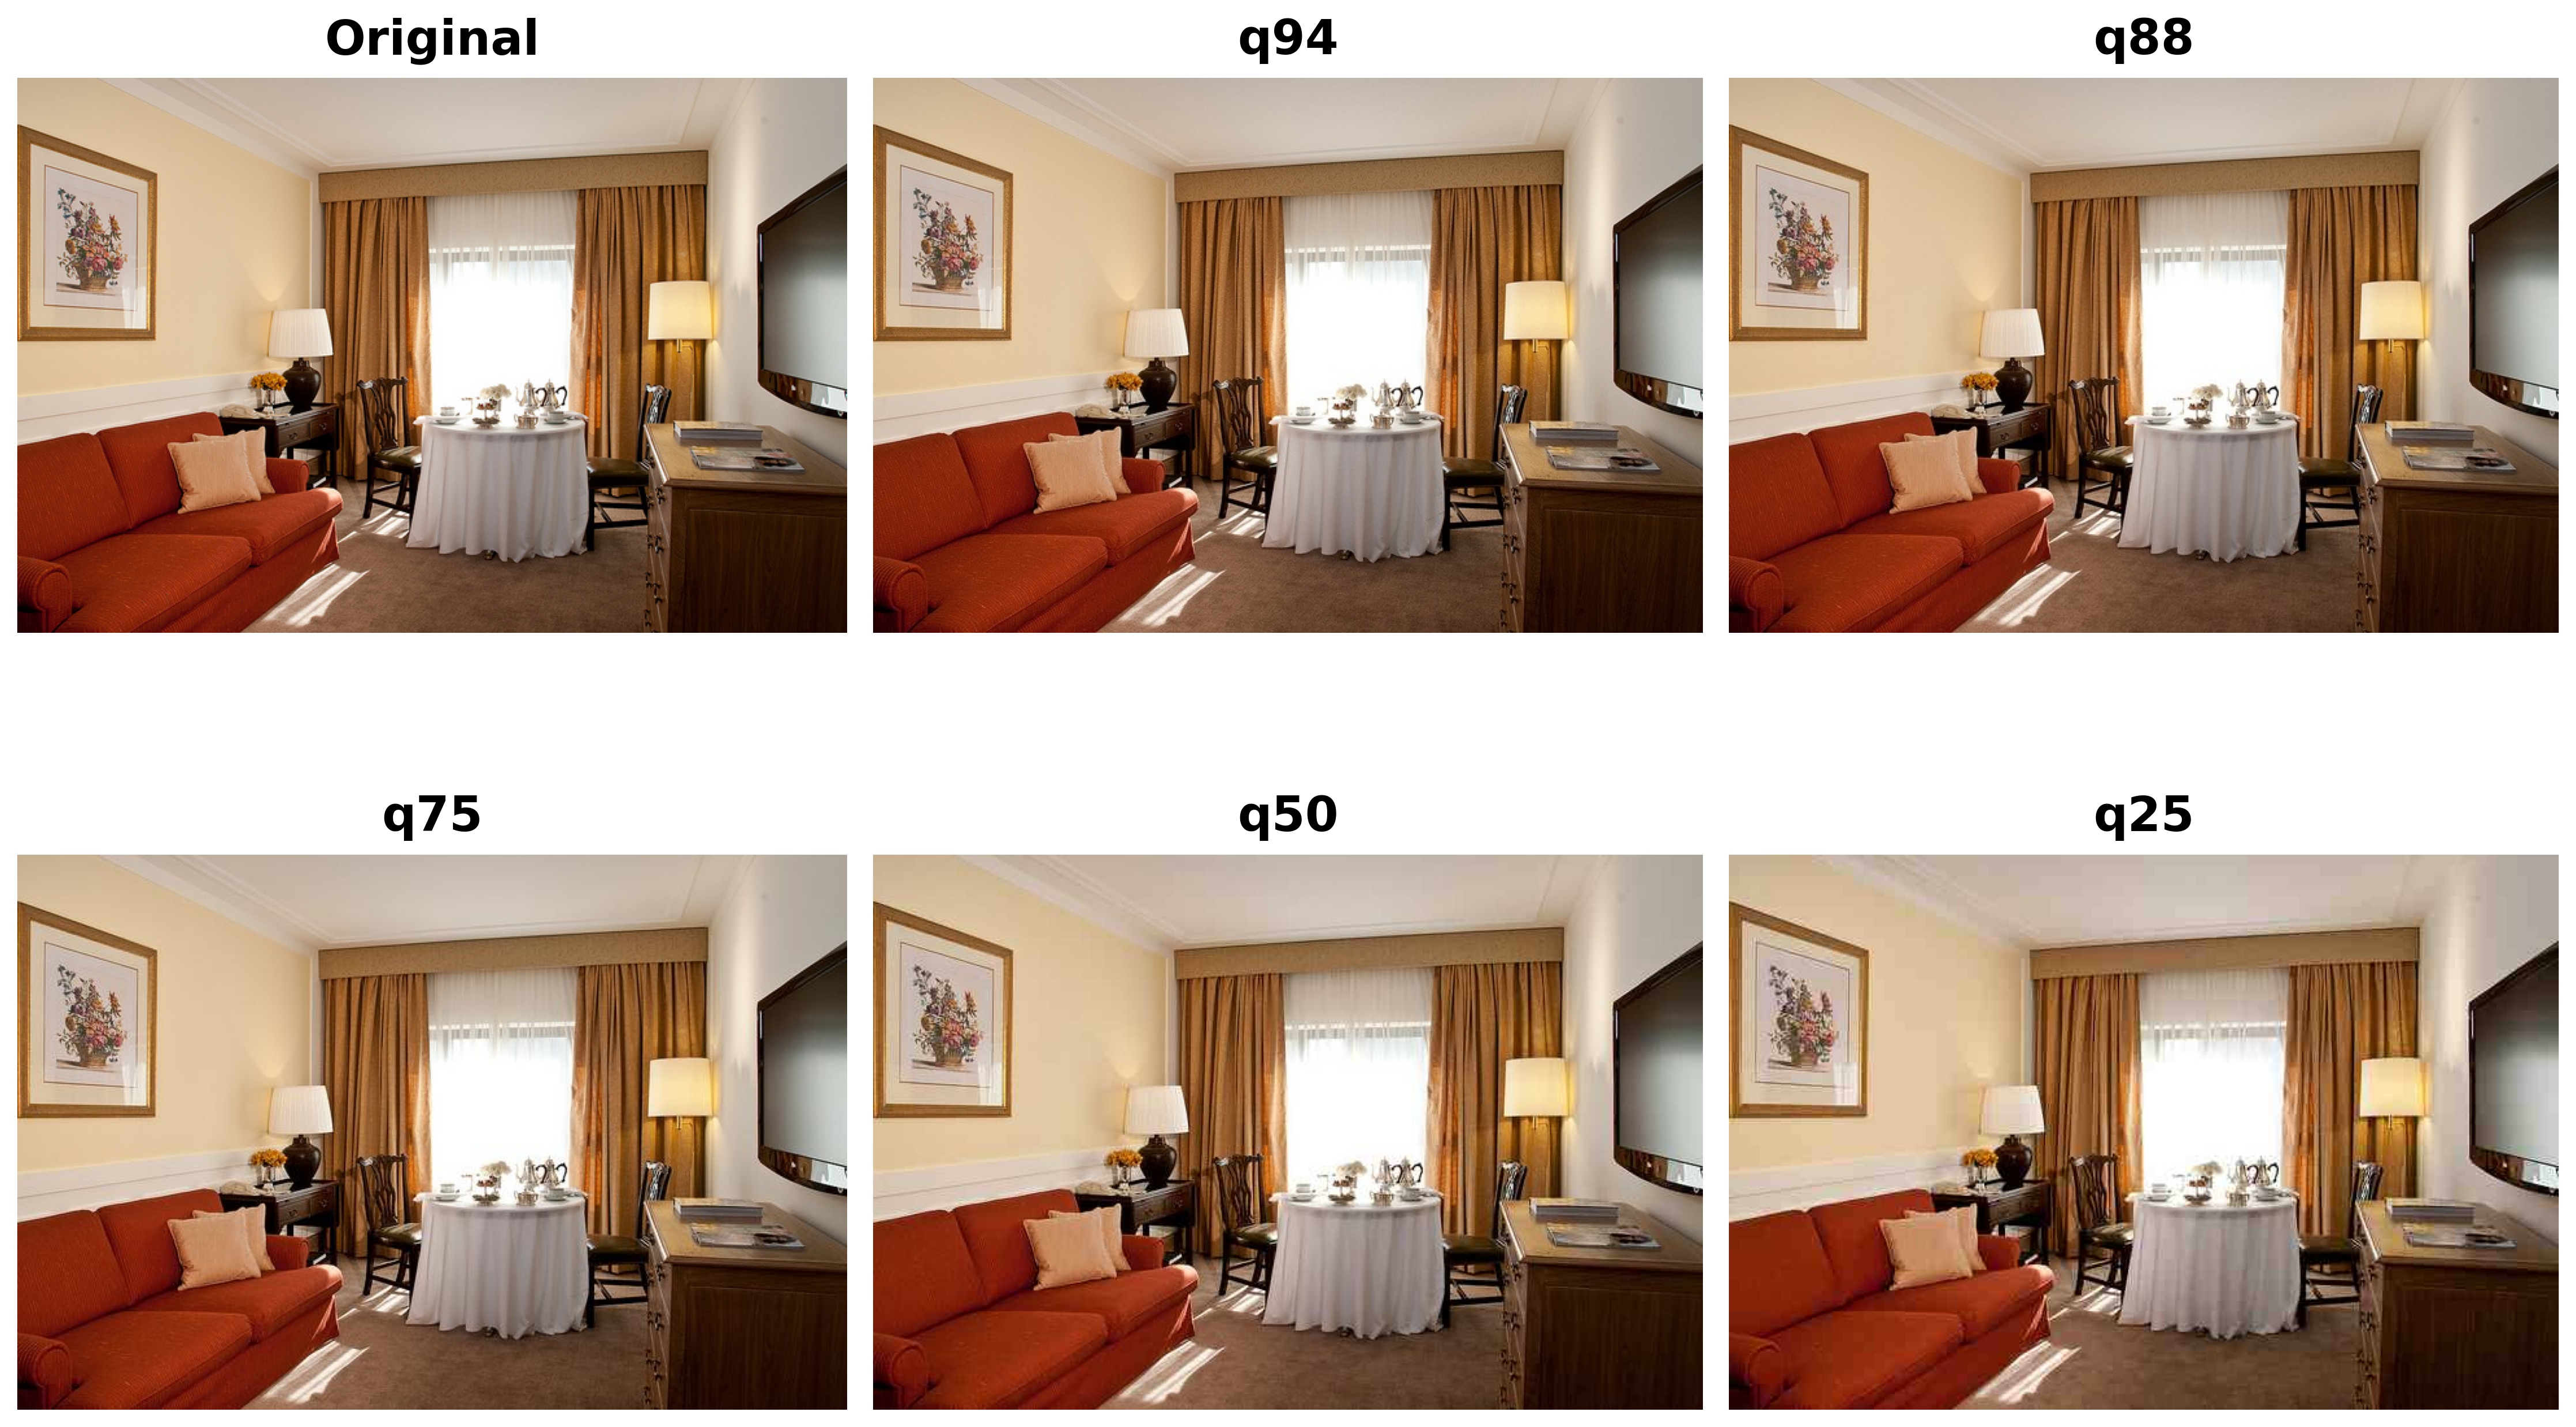
\includegraphics[width=0.75\columnwidth]{results/article_figures/fig8_jpeg_visual_degradation_grid.png}
\caption{Visual degradation examples for JPEG recompression (source, q88, q75, q25).}
\label{fig:jpeg_degrad}
\end{figure}

As observed in Fig.~\ref{fig:jpeg_degrad}, JPEG recompression introduces minor blocking and high-frequency smoothing at $q88$ and $q75$. At a severe compression level of $q25$, the $8\times8$ block boundaries become prominent and fine textures are eliminated, though the primary geometric object outlines remain intact.

The visual impact of uniform bit-depth reduction is demonstrated in Fig.~\ref{fig:bpc_degrad}.

\begin{figure}[H]
\centering
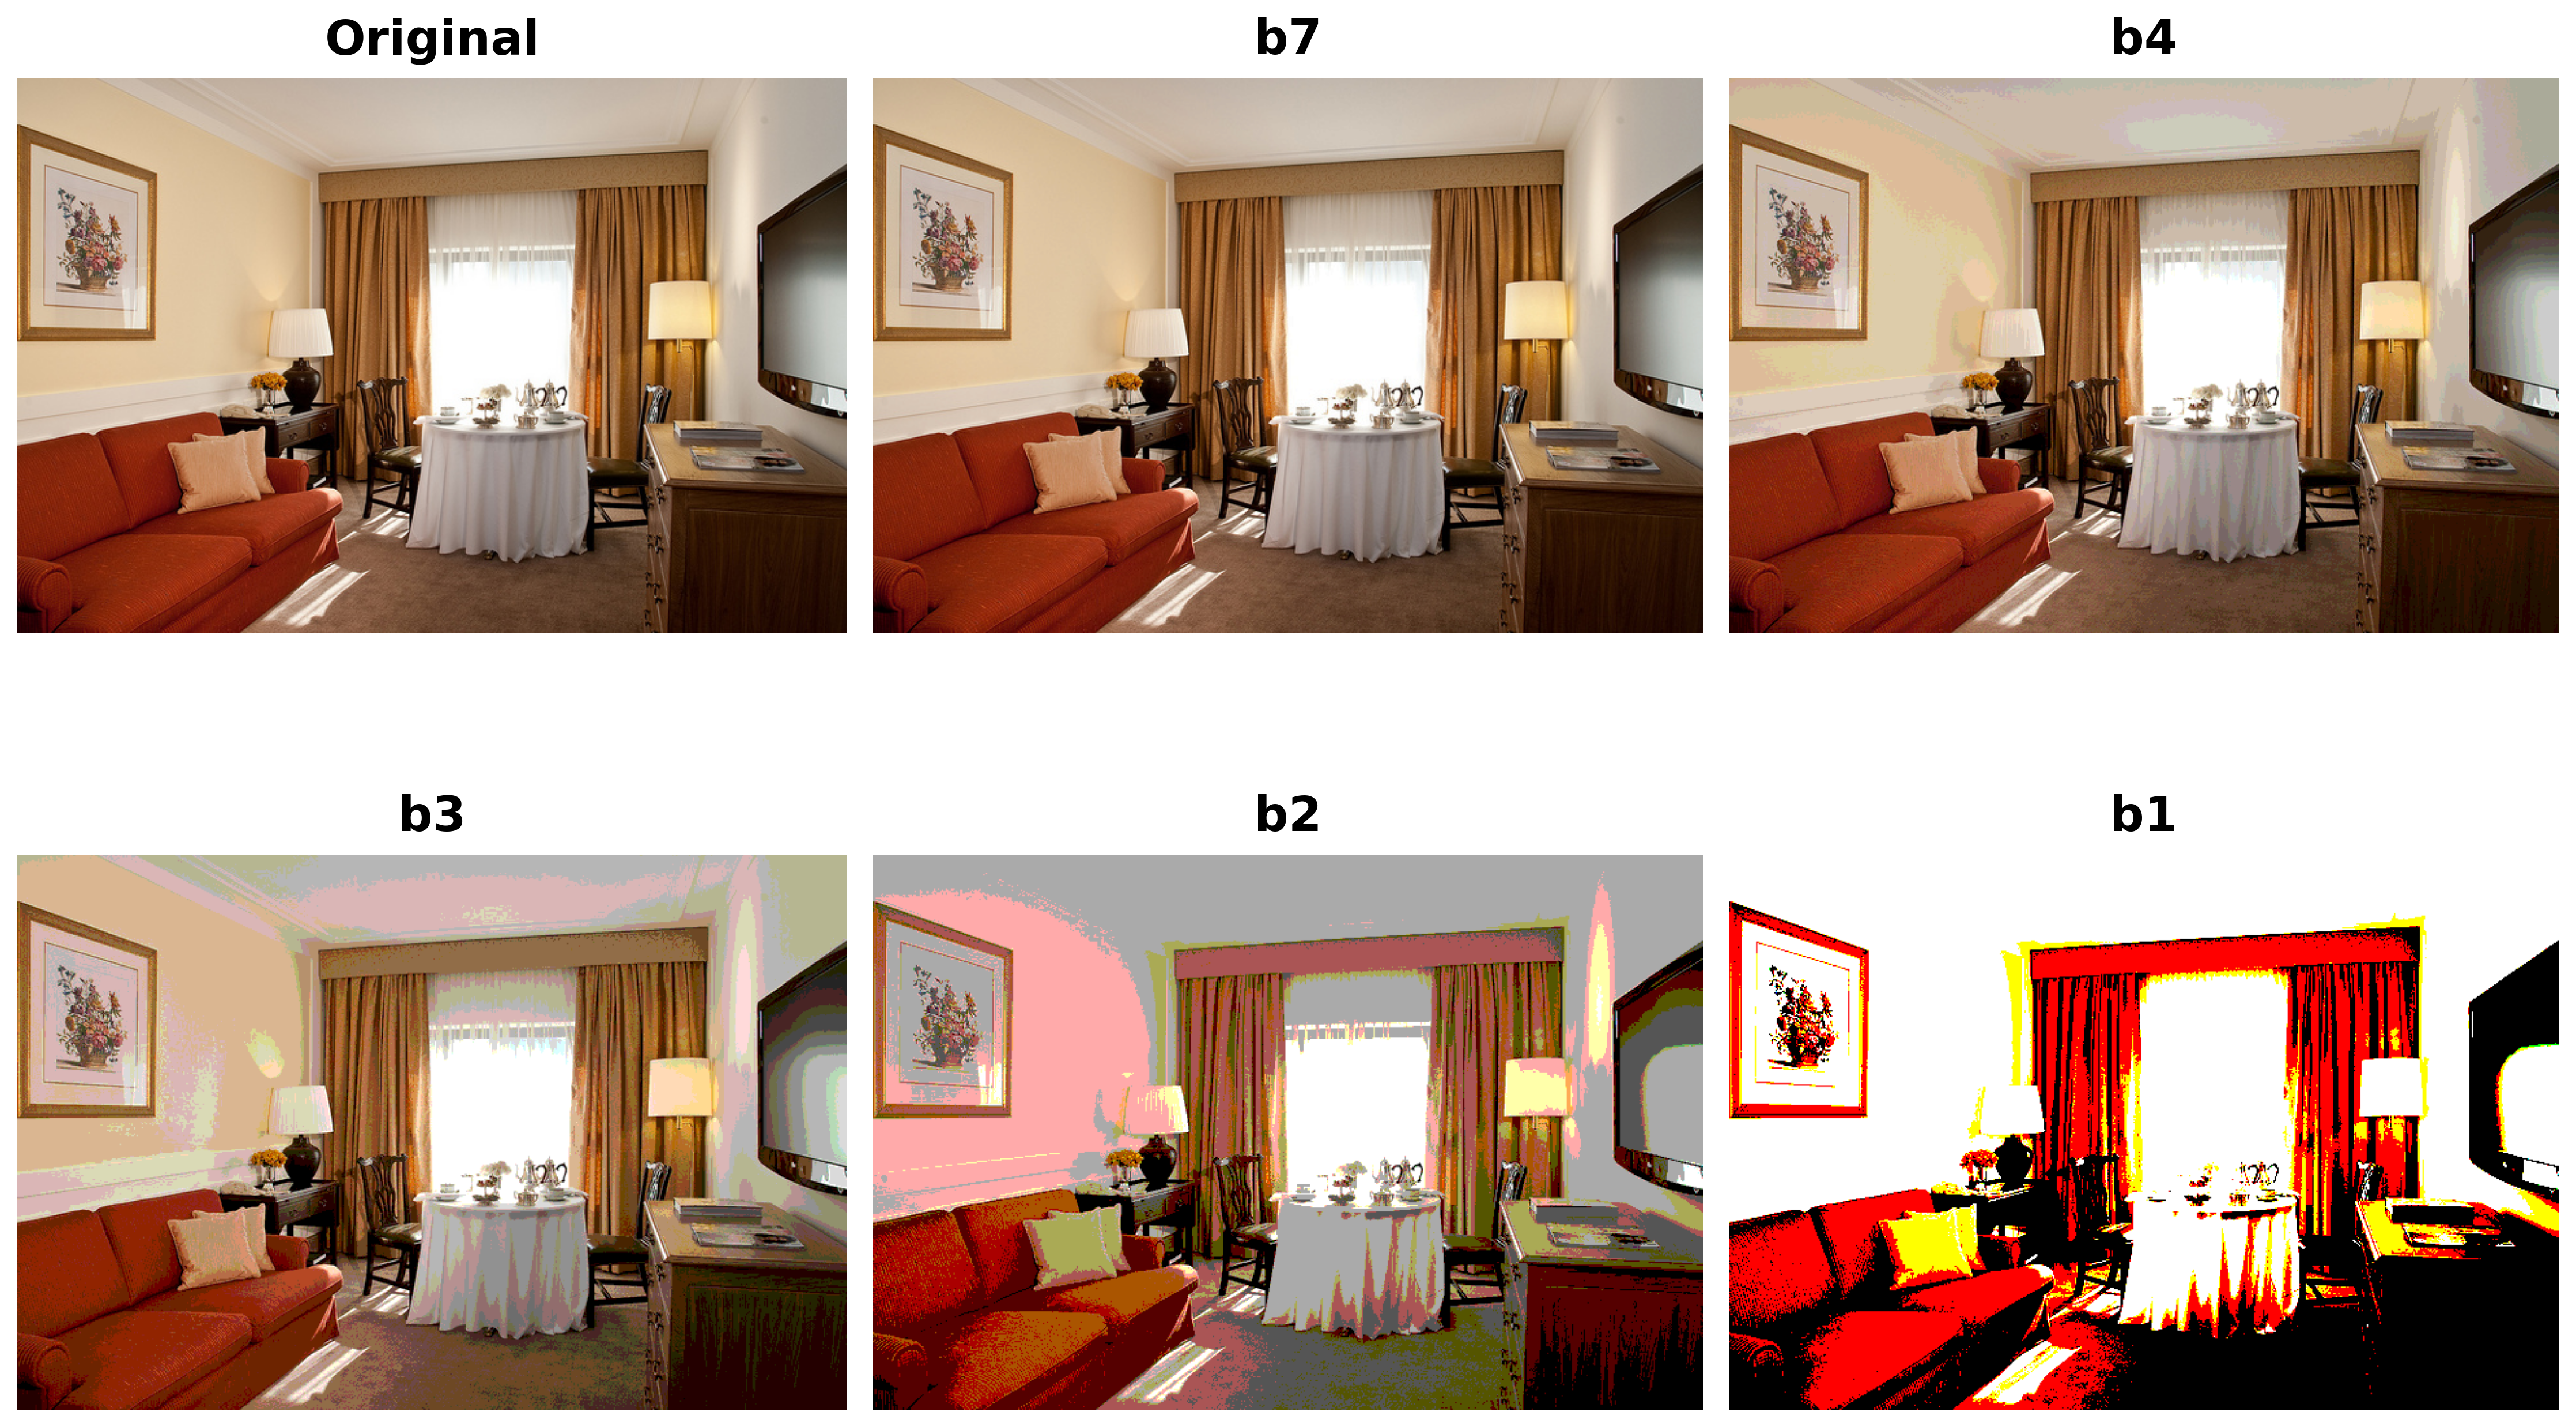
\includegraphics[width=0.75\columnwidth]{results/article_figures/fig9_bpc_visual_degradation_grid.png}
\caption{Visual degradation examples for bit-depth reduction (original decoded to PNG container, equivalent to $b8$; $b7$; $b4$; $b2$; $b1$).}
\label{fig:bpc_degrad}
\end{figure}

The $b8$ PNG control (Fig.~\ref{fig:bpc_degrad}, first panel) remains visually indistinguishable from the JPEG reference. The $b7$ and $b4$ images also maintain visual integrity, although subtle posterization becomes apparent on smooth gradients at $b4$. At lower bit depths ($b2$ and $b1$), severe tonal quantization produces high-contrast posterized patches. These artifacts disrupt the smooth amplitude transitions required by the neural network for feature extraction. 

Finally, to directly compare storage efficiency against detection quality across varying parameters, Fig.~\ref{fig:pareto_frontier} plots all non-baseline variants on a size-vs-mAP50 plane, including the corresponding Pareto frontier. The $b8$ PNG control is excluded from the frontier as it represents container-level storage inflation rather than actual quantization.

\begin{figure}[H]
\centering

\includegraphics[width=0.75\columnwidth]{results/article_figures/fig10_pareto_storage_map50.png}
\caption{Storage-detection Pareto frontier for tested JPEG and BPC variants. The $b8$ marker (diamond) denotes the PNG container control and is not part of the frontier.}
\label{fig:pareto_frontier}
\end{figure}

Mathematically, $q94$ and $b7$ lie on the Pareto frontier. However, the 0.0002 mAP50 improvement of $b7$ over the baseline falls within statistical noise limits. Accounting for such negligible metric fluctuations, the only practically viable variants on the Pareto frontier emerge from the JPEG pipeline.

\section{Discussion}
The empirical results compiled in this study provide several critical insights into the design of machine-centric digital image pipelines. Taken together, they demonstrate that different types of image degradation affect YOLOv8 in distinct ways: an equal reduction in file size does not imply equal utility for object detection, and a visually acceptable image is not necessarily the optimal input for neural network inference. Furthermore, classical metrics such as PSNR and SSIM prove insufficient for a complete assessment of image suitability in computer vision tasks. Consequently, compression methods for machine analysis must be evaluated using application-level detection metrics.

JPEG recompression demonstrates exceptional efficiency in the near-baseline and mid-range zones. Among the tested quality levels, $q88$ provides the best near-baseline trade-off it achieves a 2.02$\times$ compression ratio, halving the required storage footprint to 384.22 MB, while incurring only a 0.004 absolute mAP50 drop (a 0.77\% relative loss). In practical edge-AI deployments, switching from the source COCO JPEG baseline to $q88$ can approximately double effective storage capacity with virtually no impact on object detection accuracy. For systems operating under tighter storage or bandwidth constraints, $q75$ remains an excellent compromise, achieving 3.25$\times$ compression and reducing the dataset to 239.21 MB with only a 2.51\% relative mAP50 penalty. The slight Precision increase observed at $q88$ (0.6446 vs. 0.6347) is not accompanied by a meaningful mAP50 gain and is therefore best interpreted as a minor metric fluctuation rather than evidence of a systematic filtering benefit.

The BPC branch highlights an important architectural limitation: uniform RGB level quantization stored in a standard lossless 24-bit truecolor PNG container is highly inefficient for storage optimization under the tested pipeline. Re-encoding the decoded source JPEG as an 8-bit truecolor PNG without additional level reduction preserves baseline detection metrics (mAP50 = 0.5187) but inflates storage to 2288.66 MB. This 0.34$\times$ compression relative to the source JPEG baseline isolates a substantial container penalty before any quantization is even applied. With 7-bit level reduction, detection performance remains near baseline (0.5189 mAP50). Although removing 1 bit from the 8-bit depth discards half of the available colors per channel, this reduction fails to generate a significantly higher number of structural matches for the PNG spatial prediction algorithm. Substantial compressibility relative to the 8-bit PNG only begins to emerge at 4 bits per channel, where a 16-fold reduction in colors per channel finally yields a sufficient number of matching segments and uniform color intervals. However, even at 4 bits per channel, the PNG storage footprint (816.80 MB) remains larger than the source JPEG baseline. This PNG size behavior arises from the interaction between lossless PNG encoding---namely spatial filtering followed by DEFLATE entropy coding \cite{w3c2003}---and the spatial statistics of quantized RGB images. Uniform quantization replaces smooth gradients with step-like color intervals (posterization), which actively degrades compressibility depending on image content and filter choice. When the bit depth is lowered enough to achieve actual storage savings over the source dataset (e.g., $b3$ at 607.81 MB), the tonal quantization becomes severe. High-contrast posterized regions dominate the image, coinciding with a sharp decline in detection performance.

The results also indicate that classical full-reference quality metrics are limited predictors of deep learning performance. Comparing $b4$ and $q75$, we observe that $b4$ has a higher PSNR (34.48 dB vs. 32.29 dB) and a higher SSIM (0.9064 vs. 0.9055). To a human observer, the $b4$ image appears sharper and less distorted than the blocky $q75$ image. However, YOLOv8n achieves a higher mAP50 on $q75$ (0.5057) than on $b4$ (0.4987), while $q75$ requires 3.4$\times$ less storage (239.21 MB vs. 816.80 MB). These results suggest that YOLOv8n is more tolerant of the tested JPEG recompression artifacts than of severe RGB level quantization. A feature-level analysis would be required to establish the underlying mechanism. Consequently, PSNR and SSIM are insufficient as sole predictors of downstream detection quality across different distortion families.

To further investigate this PNG storage paradox, we conducted a supplementary storage-only experiment. Using the exact same uniform RGB level quantization from the BPC branch, each of the 5,000 val2017 images was written as an uncompressed 24-bit BMP in memory and then compressed individually with LZMA (preset 6) using the Python \texttt{lzma} module, which implements the Lempel--Ziv--Markov chain algorithm \cite{pavlov2013}. This provided an auxiliary comparison between two lossless storage pipelines, helping us assess how container structure and entropy coding interact with quantized RGB data.

Two observations followed immediately. First, the uncompressed BMP payload is effectively independent of the quantization level $b$: every variant blindly allocates three 8-bit channels per pixel before compression. Second, while per-file LZMA reduces the total size relative to BMP, it does not uniformly outperform PNG.

\begin{table}[htbp]
\centering
\caption{Storage comparison of PNG containers (main experiment) versus per-image BMP+LZMA archives (auxiliary experiment, 5,000 images). Uncompressed BMP size was approximately 4,110 MB for every tested $b$.}
\label{tab:lzma_png_storage}
\begin{tabular}{|l|r|r|r|r|}
\hline
\textbf{Variant} & \textbf{BMP raw (MB)} & \textbf{PNG (MB)} & \textbf{LZMA (MB)} & \textbf{PNG / LZMA} \\ \hline
$b7$ & 4110 & 1912.67 & 2005.76 & 0.95$\times$ \\ \hline
$b4$ & 4110 & 816.80 & 662.79 & 1.23$\times$ \\ \hline
$b3$ & 4110 & 607.81 & 400.35 & 1.52$\times$ \\ \hline
$b2$ & 4110 & 322.76 & 223.31 & 1.45$\times$ \\ \hline
$b1$ & 4110 & 165.60 & 112.35 & 1.47$\times$ \\ \hline
\end{tabular}
\end{table}

It is crucial to interpret Table~\ref{tab:lzma_png_storage} strictly as a \textit{storage-format} comparison; LZMA archives were not fed directly into YOLOv8. The practical implication is that machine-centric pipelines must jointly optimize three distinct elements: the number of bits stored per channel, the intermediate uncompressed representation, and the entropy coder. PNG exploits 2D spatial prediction, whereas LZMA relies on 1D dictionary redundancy within a byte stream. Neither approach outperforms JPEG when both storage efficiency and downstream detection metrics are prioritized.

This empirical storage paradox should not be misconstrued as evidence that all bit-depth reduction schemes are inherently inefficient. In this study, heavily quantized variants such as $b1$, which contain at most $2^3=8$ unique RGB colors, were still forced into a container that represents each pixel using three 8-bit channels before lossless compression. This introduces a severe mismatch between the theoretical bit-depth of the signal and its physical storage layout. PNG inherently supports indexed, palette-based modes capable of encoding low-cardinality images far more compactly. Consequently, a significant portion of the observed inefficiency is attributable to the container format rather than the quantization math itself. 

An analogous limitation applies to the BMP+LZMA pipeline, which expands all images to 24-bit RGB888 right before entropy coding, discarding the natural compactness of low-bit-depth signals. Direct bit-packing or sub-byte stream encoding could theoretically eliminate this pre-compression overhead, though such techniques were beyond the scope of this study.

The central insight derived from this analysis is that image compression for computer vision tasks cannot be evaluated using human visual perception or PSNR/SSIM metrics. Neural networks are highly sensitive to the \textit{type} of distortion introduced. Not all information loss is equally harmful, and compressing an image for human consumption is fundamentally different from compressing it for machine analysis. Ultimately, the choice of compression methodology must be intrinsically tied to the downstream task.

\section{Conclusion}
This study presents a task-aware evaluation of image compression and quantization strategies, conclusively demonstrating that the visual appeal of an image to a human observer does not predict its utility for automated deep learning systems.

The main findings dictate that the effectiveness of image compression for object detection tasks must be evaluated via downstream task metrics, not just visual quality scores. We found that JPEG compression and bit-depth reduction exert entirely different effects on object detection quality, even at comparable compression ratios. The structural nature of the distortions introduced is just as critical as the total volume of information lost. While moderate bit-depth reduction can preserve task-relevant information, its real-world efficiency depends entirely on the chosen storage format. 

Among the tested regimes, JPEG \textbf{q88} provides the optimal practical operating point. It halves the dataset storage size (2.02$\times$ compression) while suffering less than a 1\% relative drop in object detection accuracy ($mAP50 = 0.5147$ vs. baseline $0.5187$). For tighter operational budgets, \textbf{q75} delivers 3.25$\times$ compression with only a 2.51\% mAP50 penalty. Conversely, storing decoded images in 24-bit truecolor PNG proved highly inefficient. The $b8$ container control inflated to 2.95$\times$ the size of the source JPEG baseline without improving detection metrics, and quantized variants like $b7$ remained significantly larger than their JPEG counterparts. Finally, the consistent divergence between traditional visual quality metrics (PSNR, SSIM) and neural network task metrics (mAP) proves that human-centric evaluation is inadequate for machine vision engineering.

We acknowledge the boundary conditions of the present study: it relies on a single detector family (YOLOv8), a single benchmark dataset, and uniform RGB quantization saved via a standard 24-bit truecolor lossless PNG container. Furthermore, the JPEG branch acts as a second-order lossy recompression since the source COCO images were inherently JPEGs. Future research should investigate modern codecs such as WebP, AVIF, and JPEG XL; test the generalizability of these findings across different detector paradigms and learned machine-centric compression algorithms; and expand upon the BMP+LZMA pilot by incorporating end-to-end detection evaluation using packed bitstreams and indexed PNGs.

\begin{thebibliography}{20}

\bibitem{wallace1992}
Wallace, G. K. (1992). The JPEG still picture compression standard. \textit{IEEE Transactions on Consumer Electronics}, \textit{38}(1), xviii–xxxiv. https://doi.org/10.1109/30.125072

\bibitem{w3c2003}
World Wide Web Consortium. (2003). \textit{Portable Network Graphics (PNG) specification (second edition)} (W3C Recommendation 10 November 2003). https://www.w3.org/TR/PNG/

\bibitem{wang2004}
Wang, Z., Bovik, A. C., Sheikh, H. R., \& Simoncelli, E. P. (2004). Image quality assessment: From error visibility to structural similarity. \textit{IEEE Transactions on Image Processing}, \textit{13}(4), 600–612. https://doi.org/10.1109/TIP.2003.819861

\bibitem{hore2010}
Horé, A., \& Ziou, D. (2010). Image quality metrics: PSNR vs. SSIM. \textit{2010 20th International Conference on Pattern Recognition}, 2366–2369. https://doi.org/10.1109/ICPR.2010.579

\bibitem{zhai2020}
Zhai, G., \& Min, X. (2020). Perceptual image quality assessment: A survey. \textit{Science China Information Sciences}, \textit{63}(11), 211301. https://doi.org/10.1007/s11432-019-2757-1

\bibitem{jocher2023}
Jocher, G., Chaurasia, A., \& Qiu, J. (2023). \textit{Ultralytics YOLOv8} (Version 8.0.0) [Computer software]. https://github.com/ultralytics/ultralytics

\bibitem{redmon2016}
Redmon, J., Divvala, S., Girshick, R., \& Farhadi, A. (2016). You only look once: Unified, real-time object detection. \textit{Proceedings of the IEEE Conference on Computer Vision and Pattern Recognition (CVPR)}, 779–788. https://doi.org/10.1109/CVPR.2016.91

\bibitem{wang2023}
Wang, C.-Y., Bochkovskiy, A., \& Liao, H.-Y. M. (2023). YOLOv7: Trainable bag-of-freebies sets new state-of-the-art for real-time object detectors. \textit{Proceedings of the IEEE/CVF Conference on Computer Vision and Pattern Recognition (CVPR)}, 7464–7475. https://doi.org/10.1109/CVPR52729.2023.00721

\bibitem{lin2014}
Lin, T.-Y., Maire, M., Belongie, S. J., Hays, J., Perona, P., Ramanan, D., Dollár, P., \& Zitnick, C. L. (2014). Microsoft COCO: Common objects in context. In D. Fleet, T. Pajdla, B. Schiele, \& T. Tuytelaars (Eds.), \textit{Computer vision – ECCV 2014} (pp. 740–755). Springer. https://doi.org/10.1007/978-3-319-10602-1\_48

\bibitem{song2021}
Song, M., Choi, J., \& Han, B. (2021). Variable-rate deep image compression through spatially-adaptive feature transform. \textit{Proceedings of the IEEE International Conference on Computer Vision (ICCV)}, 2360–2369. https://doi.org/10.1109/ICCV48922.2021.00238

\bibitem{ye2023}
Ye, J., Yeo, H., Park, J., \& Han, D. (2023). AccelIR: Task-aware image compression for accelerating neural restoration. \textit{Proceedings of the IEEE/CVF Conference on Computer Vision and Pattern Recognition (CVPR)}, 17852–17861. https://doi.org/10.1109/CVPR.2023.01712

\bibitem{gandor2022}
Gandor, T., \& Nalepa, J. (2022). First gradually, then suddenly: Understanding the impact of image compression on object detection using deep learning. \textit{Sensors}, \textit{22}(3), 1104. https://doi.org/10.3390/s22031104

\bibitem{hao2022}
Hao, Y., Pei, H., Lyu, Y., Yuan, Z., Rizzo, J.-R., Wang, Y., \& Fang, Y. (2022). \textit{Understanding the impact of image quality and distance of objects to object detection performance}. arXiv preprint arXiv:2209.08237. https://doi.org/10.48550/arXiv.2209.08237

\bibitem{huang2024}
Huang, C.-H., \& Wu, J.-L. (2024). Unveiling the future of human and machine coding: A survey of end-to-end learned image compression. \textit{Entropy}, \textit{26}(5), 357. https://doi.org/10.3390/e26050357

\bibitem{piran2022}
Jamil, S., Piran, M. J., \& Rahman, M. U. (2022). Learning-driven lossy image compression: A comprehensive survey. \textit{arXiv preprint arXiv:2201.09240}. https://doi.org/10.48550/arXiv.2201.09240

\bibitem{heckbert1982}
Heckbert, P. S. (1982). Color image quantization for frame buffer display. \textit{Proceedings of the 9th Annual Conference on Computer Graphics and Interactive Techniques (SIGGRAPH ’82)}, 297–307. https://doi.org/10.1145/800064.801294

\bibitem{floyd1976}
Floyd, R. W., \& Steinberg, L. (1976). An adaptive algorithm for spatial grey scale. \textit{Proceedings of the Society of Information Display}, \textit{17}(2), 75–77.

\bibitem{jacob2018}
Jacob, B., Kligys, S., Chen, B., Zhu, M., Tang, M., Howard, A., Adam, H., \& Kalenichenko, D. (2018). Quantization and training of neural networks for efficient integer-arithmetic-only inference. \textit{Proceedings of the IEEE Conference on Computer Vision and Pattern Recognition (CVPR)}, 2704–2713. https://doi.org/10.1109/CVPR.2018.00291

\bibitem{han2016}
Han, S., Mao, H., \& Dally, W. J. (2016). Deep compression: Compressing deep neural networks with pruning, trained quantization and Huffman coding. \textit{International Conference on Learning Representations (ICLR)}. https://arxiv.org/abs/1510.00149

\bibitem{pavlov2013}
Pavlov, I. (2013). \textit{LZMA SDK} (Version 9.20) [Computer software]. https://www.7-zip.org/sdk.html

\end{thebibliography}

\end{document}
